\chapter{Testing and Evaluation}
\label{chap:eval}
\lhead{\emph{Project Testing}}
The goal of this chapter is an objective evaluation of the final AI Docker Linter \& Optimizer system. The evaluation focuses on quantitative metrics to assess the system's effectiveness, accuracy, and performance. Where applicable, a comparative analysis is performed against Hadolint, a widely used static analysis tool for Dockerfiles. The testing utilizes a benchmark dataset of Dockerfiles to evaluate the system's ability to achieve its core objectives in realistic scenarios.

\section{Metrics}
\label{sec:eval_metrics}
To evaluate the system comprehensively, the following key metrics were identified and measured:

\begin{itemize}
    \item \textbf{Optimization Effectiveness:}
        \begin{itemize}
            \item \textbf{Build Success Rate (\%):} The percentage of Dockerfiles from the test set for which the optimized version could be successfully built into a Docker image. This measures the reliability and correctness of the optimization component.
            \item \textbf{Average Image Size Reduction (\%):} For successfully optimized Dockerfiles built, the average percentage reduction in final image size compared to the original Dockerfile image size. This quantifies the primary goal of reducing image bloat.
        \end{itemize}
    \item \textbf{Linter Accuracy (Comparison with Hadolint):} To evaluate the AI-driven linter component, its ability to identify potential issues (violations of best practices) was compared with Hadolint using standard classification metrics.
        \begin{itemize}
            \item \textbf{Precision:} The proportion of issues identified (by the linter) that were actual issues (true positives) out of all problems identified by the linter (true positives + false positives). \( \text{Precision} = \frac{TP}{TP + FP} \)
            \item \textbf{Recall:} The proportion of actual issues that were correctly identified by the linter (true positives) out of all actual issues present (true positives + false negatives). \( \text{Recall} = \frac{TP}{TP + FN} \)
            \item \textbf{F1-Score:} The harmonic mean of Precision and Recall, providing a single measure of the linter's accuracy. \( \text{F1 Score} = 2 \times \frac{\text{Precision} \times \text{Recall}}{\text{Precision} + \text{Recall}} \)
        \end{itemize}
        These metrics were calculated for both the custom AI linter and Hadolint based on a manually annotated ground truth for the Dockerfile test set.
    \item \textbf{Performance:}
        \begin{itemize}
            \item \textbf{Average Analysis Duration (seconds):} The average time taken by the system to fully analyze and process a single Dockerfile (including linting and optimization suggestion).
            \item \textbf{Analysis Duration vs. Dockerfile Size:} Correlation between the analysis duration and the size (number of lines) of the input Dockerfile. This helps understand the scalability and performance characteristics of the tool.
        \end{itemize}
\end{itemize}

\section{System Testing}
\label{sec:eval_setup}
The evaluation was conducted using a defined experimental setup to ensure reproducible and objective measurements.

\begin{itemize}
    \item \textbf{Dataset:} A benchmark set of 7 Dockerfiles (\texttt{testing/Dockerfiles\_set/}) was used as input for the evaluation. This set was chosen to represent a variety of common use cases and complexities. [\emph{Optional: Add more detail here if you know the origin or specific characteristics of this dataset, e.g., "sourced from popular open-source projects" or "specifically crafted to test various Dockerfile instructions."}]
    \item \textbf{Experimental Process:}
        \begin{enumerate}
            \item Each Dockerfile in the dataset was processed by the AI Docker Linter \& Optimizer system.
            \item For optimization evaluation, the tool generated an optimized version of the Dockerfile. An attempt was made to build a Docker image from both the original and the optimized Dockerfile. Image sizes were recorded, and the build success/failure was noted.
            \item For linter evaluation, both the custom AI linter and Hadolint were run on the original Dockerfiles. Their outputs were compared against a pre-defined ground truth (manual annotation of actual issues) to calculate Precision, Recall, and F1-Score.
            \item The time taken for the AI system to analyze each Dockerfile was recorded.
            \item The number of lines in each Dockerfile was recorded to analyze correlation with processing time.
        \end{enumerate}
    \item \textbf{Tooling:} The experiments were automated using Python scripts. The primary script, \texttt{testing/evaluate\_results.py}, orchestrated the processing of Dockerfiles, interaction with the AI tool, execution of Hadolint, Docker image builds, and collection of raw data. The script \texttt{testing/generate\_graphs.py} was used subsequently to process the raw data (stored in \texttt{testing/evaluation\_summary.json}) and generate visualizations.
\end{itemize}

\section{Results}
\label{sec:eval_results}
The evaluation yielded quantitative results across the defined metrics, summarized below. The raw aggregated data can be found in \texttt{testing/evaluation\_summary.json}.
\begin{itemize}
    \item \textbf{Optimization Effectiveness (Issue Counts):} A comparison based on the number of issues resolved, unresolved, and newly introduced revealed the following:
        \begin{itemize}
            \item \textbf{Resolved Issues:} The Custom Method resolved 53 issues, while ChatGPT-4o resolved 52 issues. Both methods showed comparable effectiveness in resolving existing issues.
            \item \textbf{Unresolved Issues:} The Custom Method left 0 issues unresolved, while ChatGPT-4o left 1 issue unresolved.
            \item \textbf{New Issues Introduced:} The Custom Method introduced 9 new issues during optimization, significantly fewer than the 29 new issues introduced by ChatGPT-4o.
            \item Overall, while both methods were effective at resolving issues, the Custom Method introduced considerably fewer new problems.
        \end{itemize}
        Figure \ref{fig:opt_eff} illustrates this comparison.
         \begin{figure}[ht]
            \centering
            % Ensure the image path 'testing/optimization_comparison.png' exists
            % or update it to the correct path for Figure 6.1
            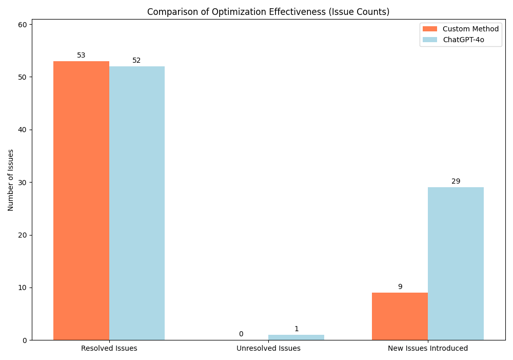
\includegraphics[width=0.8\textwidth]{Figures/Picture3_comparisonAI.png}
            \caption{Comparison of Optimization Effectiveness (Issue Counts): Custom Method vs. ChatGPT-4o.}
            \label{fig:opt_eff}
        \end{figure}

% The closing \end{itemize} should be present from the parent list structure
% \end{itemize}


     \item \textbf{Performance:}
        \begin{itemize}
            \item The \textbf{Average Analysis Duration} per Dockerfile was \textbf{64.80 seconds}. 
            \item One file analysis took significantly longer (303 seconds), which substantially skews this average. The median duration or an average calculated without this outlier might offer a more representative measure of typical performance.
            \item Figure \ref{fig:time_corr} illustrates the relationship between the analysis duration and the Dockerfile size (in lines). The plot shows variability in analysis time, particularly highlighting the outlier, and allows for visual assessment of any correlation between file size and processing time. % You can add specific observations here, e.g., "showing a weak positive correlation" or "indicating increased variance for larger files" once you interpret the graph.
        \end{itemize}
         \begin{figure}[ht]
            \centering
            % Ensure the path 'Figures/Picture3_size.png' is correct
            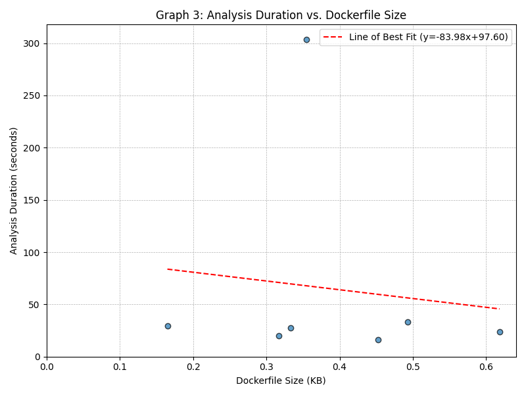
\includegraphics[width=0.8\textwidth]{Figures/Picture3_size.png} 
            \caption{Analysis Duration vs. Dockerfile Size (Lines).}
            \label{fig:time_corr}
        \end{figure}

\end{itemize}

\textbf{Threats to Validity:}
Potential threats to the validity of these results include:
\begin{itemize}
    \item \textbf{Dataset Size and Representativeness:} The evaluation used a limited set of 7 Dockerfiles. A larger, more diverse dataset might yield different average results or reveal edge cases not encountered.
    \item \textbf{Ground Truth Accuracy:} The linter accuracy metrics depend on the correctness and completeness of the manual annotation (ground truth) used for comparison. Any errors in annotation would affect the calculated Precision, Recall, and F1-Scores.
    \item \textbf{Build Environment Consistency:} Docker build processes can sometimes be affected by caching or network conditions, although efforts were made to ensure a consistent environment for comparing original and optimized builds.
    \item \textbf{Complexity of Analysis Task:} The performance metrics, particularly analysis time, are specific to the complexity of the tasks performed by this specific AI model and optimization logic. Different approaches might have different performance characteristics.
\end{itemize}
These factors should be considered when interpreting the results. A more detailed discussion follows in Chapter 5.
